\subsubsection{Funktionsweise}

Bei der Bilderzeugung, ausgehend von Szenen, welche viel Geometrie beinhalten bzw. bei Szenen 
die generelle BRDF's verwenden eignet sich der \nameref{ch:Content1:sec:PathTracer}.
Der \nameref{ch:Content1:sec:PathTracer} ist in Hinsicht der Beleuchtung komplett. Deshalb lässt sich damit
\textit{Global Illumination} erreichen. Der hier verwendete \nameref{ch:Content1:sec:PathTracer} in 
\cite{Benty18} verwendet eine klassische Umsetzung.\par
Der Path Tracer beruht auf Erkenntnisse der Lösung der allgemeinen Rendergleichung.\nameref{eq:Allgemeine Rendergleichung}

\begin{equation}\label{eq:Allgemeine Rendergleichung}
    I(x,{x}^{'}) = g(x,{x}^{'}) * \biggl[\epsilon(x,{x}^{'}) + 
    \int_{S}^{} \rho(x,{x}^{'},{x}^{''})
    I({x}^{'},{x}^{''}d{x}^{''})\biggr] 
\end{equation}

Sie beschreibt den Energietransport \textit{I} von einem Punkt ${x}^{'}$
zu einem Punkt x. Dabei ist ein maßgebender Faktor der Geometrieterm \textit{g},
der die relative Lage der beiden Punkte zueinander im Raum beschreibt.
Ein weiterer Faktor ist die Abstrahlung \textit{$\epsilon$} von ${x}^{'}$ nach x. 
Beeinflusst wird der Energiefluss auch durch
die bidirektionale Verteilungsfunktion \textit{$\rho$}, welche Aufschluss über
das einfallende Licht von einem Punkt ${x}^{''}$ über ${x}^{'}$ zu x gibt.\par
Die Schlussfolgerung aus dieser Gleichung \nameref{eq:Allgemeine Rendergleichung} ist: Die transportierte
Intensität von einem Licht zu einem Anderen ist die Summe des ausgestrahlten Lichts 
und das ausgestrahlte Licht zu x von allen anderen Oberflächen.

Ausgehend von der Rendergleichung \nameref{eq:Allgemeine Rendergleichung} lässt sich
die vollständige Transportgleichung\nameref{eq:vollständige Transportgleichung} des \nameref{ch:Content1:sec:PathTracer}
beschreiben.
Wie in \cite{marschner2009fundamentals} beschrieben wird ausgehend von der vollständigen Transportgleichung
\nameref{eq:vollständige Transportgleichung}

\begin{equation}\label{eq:vollständige Transportgleichung}
    L_s(k_0) = L_e(k_0) + \int_{all(k_i)}^{} \rho(k_i, k_0)*L_f(k_i)*cos(\theta_i)d\theta_i
\end{equation}

der vollständige Lichttransport beschrieben. Man kann deutlich die Ähnlichkeit
zu \nameref{eq:Allgemeine Rendergleichung} erkennen. Wir haben den Emissionsterm, die relative Lage der 
Punkte zueinander und die bidirektionale Verteilungsfunktion welche den Energietransport
beeinflussen.

\begin{figure}[H]
    \centering
    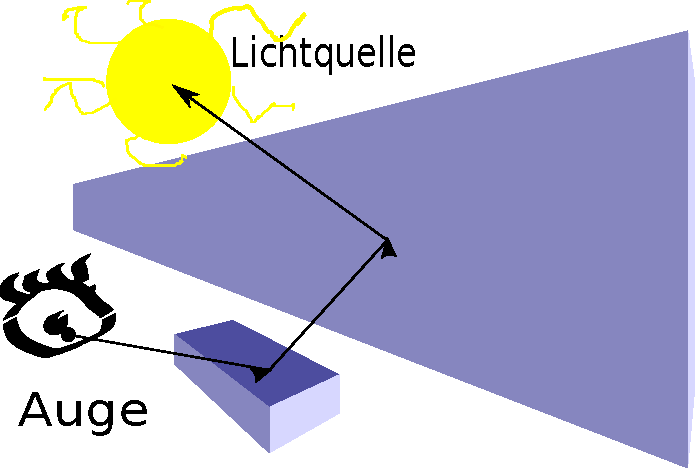
\includegraphics[width=0.7\linewidth]{content/PathTracer/Bilder/Grundkonzept_path_tracing.pdf}
    \label{pic::Grundkonzept Path Tracing}
    \caption{Grundkonzept path tracer}
\end{figure}

\subsubsection{Monte-Carlo-Integration}
Mit der Monte Carlo Integration approximieren wir die Rendergleichung.\par 
Bei gegebener Dimensionalität n des Renderintegrals und der 
Wahrscheinlichkeitsdichtefunktion $\rho(x_i)$
\cite{KK02}

\begin{equation}\label{eq:Monte-Carlo}
    E\biggl[\frac{1}{k}\sum_{i=1}^{k}\frac{f(X_{i}}{\rho(X_{i})})\biggl] = \int_{[0,1]^{n}}f(x)dx
\end{equation}

Dabei wird das n-dimensionale Integral\nameref{eq:vollständige Transportgleichung} approximiert. Die Dichtefunktion $\rho(x_i)$ 
beschreibt deutet an, dass hierbei die Stichproben auch nicht-uniform 
genommen werden können. Varianzreduktionsmethoden machen sich diese Dichtefunktion zu Nutze um 
ein besseres Ergebnis zu bekommen.
\cite{caflisch_1998}
Konvergenzrate, unabhängig von der Dimension unseres Tracers.\textit{O}($N^{-\frac{1}{2}}$).
Sie ist robust, das heißt Exaktheit hängt nur vom ungenauesten Parameter ab. Eine Variante des Verfahrens, 
Monte Carlo Quadratur, wird mit quasi zufälligen Sequenzen \nameref{ch:Content1:sec:QuasiRandomSequences}, 
welche eine niedrige Abweichung aufweisen, durchgeführt. Laufzeit quasi-Monte Carlo \textit{O}(($\log N)^{k}N^{-1}$).
Um die Konvergenzrate zu steigern liegen eine Reihe von Varianzreduktionsmethoden vor.

Abseits dieser herkömmlichen Strategien zeigen wir hier die Steigerung der 
visuellen Qualität durch blue noise Fehlerverteilung im Bildraum.

\begin{equation}\label{eq:Monte-Carlo-Varianz}
    V[X] = E\biggl[(X-E[X])^{2}\biggl] = E[X^{2}]
    - E[X]^{2}
\end{equation}

Die Varianz \nameref{eq:Monte-Carlo-Varianz} ist ein quadratischer Fehler.


\begin{figure}[H]\label{pic:Weisses Rauschen Tracer}
    \centering
    \begin{minipage}[t]{0.45\linewidth}
        \centering
        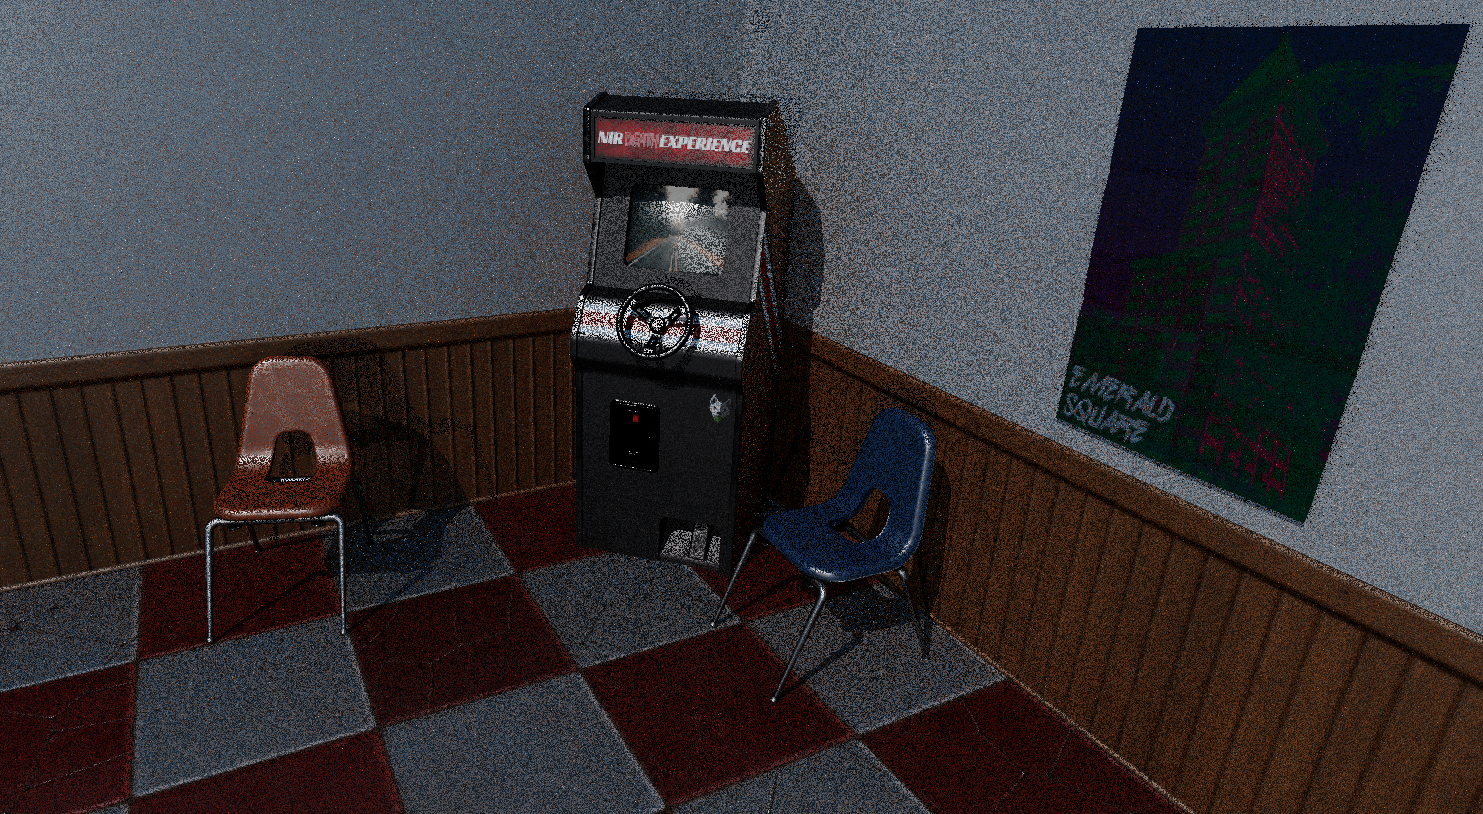
\includegraphics[width=\linewidth]{content/PathTracer/Bilder/WeissesRauschenSzene.png}
        \caption{Szene mit Weißem Rauschen}
    \end{minipage}
    \hfill
    \begin{minipage}[t]{0.45\linewidth}
        \centering
        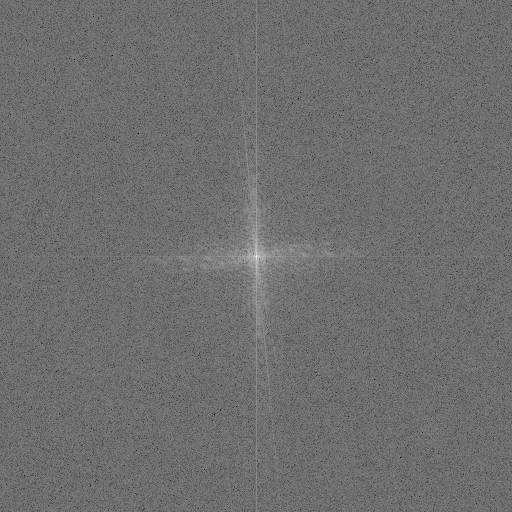
\includegraphics[width=\linewidth]{content/PathTracer/Bilder/FFT_Ausschnitt2.png}
        \caption{FFT des Ausschnitts}
    \end{minipage}
\end{figure}


\subsubsection{DirectX Raytracing}
Für besseres Verständnis möchte ich hier eine Einführung in das Path Tracing\cite{Benty18} mit Hilfe der
neuen DirectX-Schnittstelle geben.

\begin{figure}[H]
    \centering
    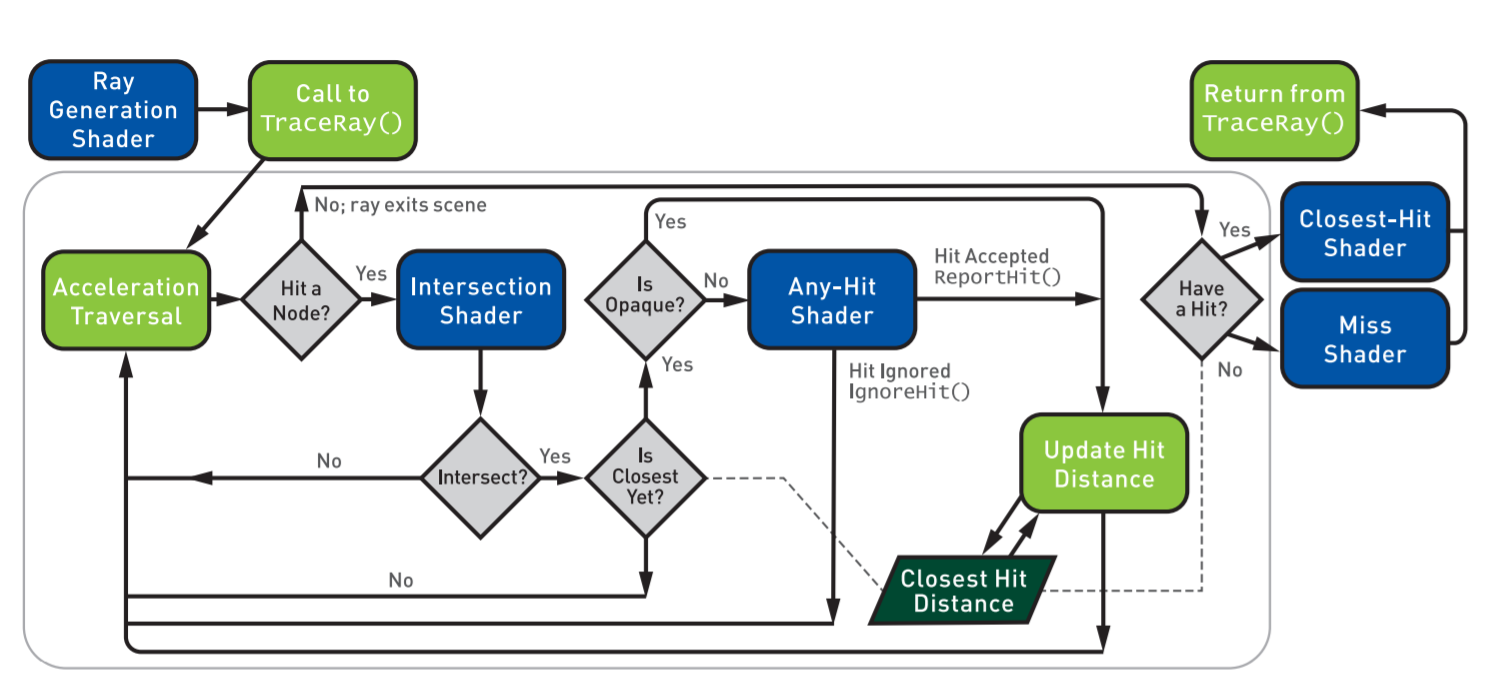
\includegraphics[width=\linewidth]{content/PathTracer/Bilder/DirectXRaytracingPipeline.png}
    \label{pic::DirectXRaytracing-Pipeline}
    \caption{DirectX Raytracing Pipeline aus \cite{Haines2019}}
\end{figure}

In der obigen Übersicht lässt sich der Start der neuen Pipeline erkennen, der \textbf{Ray Generation
shader}. Von hier aus werden Rays gestartet \textbf{TraceRay()}.
\textbf{Intersection shader} führt die Schnittpunktberechnungen durch.
\textbf{Any-hit shaders} erlauben klassische "Discards" oder informieren
über einen korrekten Schnitt. Der \textbf{Closest-hit shader} führt den
konkreten, nähsten Schnitt für jeden Strahl durch.
Der \textbf{miss shader} wird immer dann ausgeführt, wenn ein Strahl die
Szenengeometrie nicht schneidet. Kann also für das Nachschauen in einer 
Environment Map verwendet werden. Im Folgenden \nameref{alg:Path Tracer Konzept}
nochmal vereinfacht in Pseudocode dargestellt, wobei die entsprechenden shader
im jeweiligen Codeabschnitt markiert sind.

\begin{algorithm}[H]
    \caption{Was macht ein Path Tracer}
    \begin{algorithmic}[1]
        \Procedure{Trace Path}{$BVH$}\Comment{verfolge Pfad durch Szene}
        \For{(x,y) $\in$ frame}
        \State nähesterSchnittpunkt;
        \State strahl = verschiesseStrahlInPixel(x,y); // \textbf{ray generation shader}
        \For{blatt = bekommeBVHBlatt()}
        \State schnittpunkt = schneideGeometrie(strahl, blatt); //\textbf{Intersection shader}
        \If{schnittpunkt $\leq$ nähesterSchnittpunkt}
        \State aktualisiereNähestenSchnittpunkt();
        \EndIf
        \EndFor
        \If{Schnittpunkt gefunden}
        \State frame(x,y) = gebeFarbe(strahl,nähesterSchnittpunkt); //\textbf{closest-hit shader}
        \Else
        \State frame(x,y) = Umgebungskarte(x,y);//\textbf{miss shader}
        \EndIf
        \EndFor
        \EndProcedure
    \end{algorithmic}
    \label{alg:Path Tracer Konzept}
\end{algorithm}




